\documentclass{article}
\usepackage[utf8]{inputenc}
\usepackage{amsmath}
\usepackage{graphicx}
\usepackage{booktabs}
\usepackage{listings}
\usepackage{xcolor}
\usepackage{float} % Required for strict image placement [H]
\usepackage{geometry}
\geometry{a4paper, margin=1in}
\graphicspath{ {./Pictures/} }

% Setup for Python code formatting
\lstset{
    language=Python,
    basicstyle=\ttfamily\small,
    keywordstyle=\color{blue},
    stringstyle=\color{red},
    commentstyle=\color{green!60!black},
    numbers=left,
    numberstyle=\tiny,
    stepnumber=1,
    numbersep=8pt,
    backgroundcolor=\color{gray!10},
    showstringspaces=false,
    breaklines=true,
    frame=single
}

\begin{document}

\section*{Q1: Integral-Slot Winding Design}

\noindent
\textbf{Machine Parameters:} 3-phase, 6-pole, 72-slot, double-layer winding. \\
\textbf{Base Calculations:}
\begin{itemize}
    \item Slots per pole per phase ($q$): $q = \frac{72}{6 \cdot 3} = 4 \text{ slots/pole/phase}$
    \item Electrical slot angle ($\alpha$): $\alpha = \frac{3 \cdot 360^\circ}{72} = 15^\circ \text{ electrical}$
\end{itemize}

\hrulefill

\subsection*{1. Winding Diagram Layout (One Pole-Pair)}

The standard phase sequence is $A, -C, B, -A, C, -B$. With $q=4$, each phase band occupies 4 slots. Below are the double-layer winding distributions for the first 24 slots (representing exactly one pole-pair).

\subsubsection*{Full-Pitched Winding (Pitch = 12 Slots)}
The coil spans exactly one pole pitch. The upper and lower layers in each slot belong to the same phase.

\vspace{0.3cm}
\noindent
\resizebox{\textwidth}{!}{
\begin{tabular}{|l|*{24}{c|}}
\hline
\textbf{Slot} & \textbf{1} & \textbf{2} & \textbf{3} & \textbf{4} & \textbf{5} & \textbf{6} & \textbf{7} & \textbf{8} & \textbf{9} & \textbf{10} & \textbf{11} & \textbf{12} & \textbf{13} & \textbf{14} & \textbf{15} & \textbf{16} & \textbf{17} & \textbf{18} & \textbf{19} & \textbf{20} & \textbf{21} & \textbf{22} & \textbf{23} & \textbf{24} \\ \hline
\textbf{Top} & A & A & A & A & -C & -C & -C & -C & B & B & B & B & -A & -A & -A & -A & C & C & C & C & -B & -B & -B & -B \\ \hline
\textbf{Bot} & A & A & A & A & -C & -C & -C & -C & B & B & B & B & -A & -A & -A & -A & C & C & C & C & -B & -B & -B & -B \\ \hline
\end{tabular}
}

\subsubsection*{11/12 Short-Pitched Winding (Pitch = 11 Slots)}
Shortening the pitch by 1 slot shifts the bottom layer relative to the top layer, creating mixed-phase slots.

\vspace{0.3cm}
\noindent
\resizebox{\textwidth}{!}{
\begin{tabular}{|l|*{24}{c|}}
\hline
\textbf{Slot} & \textbf{1} & \textbf{2} & \textbf{3} & \textbf{4} & \textbf{5} & \textbf{6} & \textbf{7} & \textbf{8} & \textbf{9} & \textbf{10} & \textbf{11} & \textbf{12} & \textbf{13} & \textbf{14} & \textbf{15} & \textbf{16} & \textbf{17} & \textbf{18} & \textbf{19} & \textbf{20} & \textbf{21} & \textbf{22} & \textbf{23} & \textbf{24} \\ \hline
\textbf{Top} & A & A & A & \textbf{A} & -C & -C & -C & \textbf{-C} & B & B & B & \textbf{B} & -A & -A & -A & \textbf{-A} & C & C & C & \textbf{C} & -B & -B & -B & \textbf{-B} \\ \hline
\textbf{Bot} & A & A & A & \textbf{-C} & -C & -C & -C & \textbf{B} & B & B & B & \textbf{-A} & -A & -A & -A & \textbf{C} & C & C & C & \textbf{-B} & -B & -B & -B & \textbf{A} \\ \hline
\end{tabular}
}

\subsection*{2. Winding Factor Calculations}

To calculate the winding factor $K_{wn}$ for the fundamental ($n=1$), 3rd harmonic ($n=3$), and 5th harmonic ($n=5$), a Python script was utilized. The winding factor is the product of the distribution factor $K_{dn}$ and the pitch factor $K_{pn}$.

\begin{align*}
    K_{dn} &= \frac{\sin(n \cdot q \cdot \alpha / 2)}{q \cdot \sin(n \cdot \alpha / 2)} \\
    K_{pn} &= \sin\left(\frac{n \cdot \lambda}{2}\right) \quad \text{(where $\lambda$ is the electrical coil pitch)}
\end{align*}

\subsubsection*{Python Script}
\begin{lstlisting}
import math

slots = 72
pole_pairs = 3
phases = 3
layers = 2

# slots per pole per phase
q = slots / (2 * pole_pairs * phases)

# electrical slot angle in radians (alpha)
alpha = pole_pairs * 2 * math.pi / slots

# --- Distribution Factor Function ---
def calc_kd(n_harmonic):
    return math.sin(n_harmonic * q * alpha / 2) / (q * math.sin(n_harmonic * alpha / 2))

Kd1 = calc_kd(1)
Kd3 = calc_kd(3)
Kd5 = calc_kd(5)

# --- Pitch Factor Function ---
def calc_kp(n_harmonic, slots_spanned):
    # lambda is the electrical angle of the spanned slots
    lambda_rad = slots_spanned * alpha
    return math.sin(n_harmonic * lambda_rad / 2)

# Full Pitch (spans exactly 1 pole pitch = 12 slots)
Kfp1 = calc_kp(1, 12)
Kfp3 = calc_kp(3, 12)
Kfp5 = calc_kp(5, 12)

# Short Pitch 11/12 (spans 11 slots)
Ksp1 = calc_kp(1, 11)
Ksp3 = calc_kp(3, 11)
Ksp5 = calc_kp(5, 11)

# --- Winding Factor (Kw = Kd * Kp) ---
Kfw1, Kfw3, Kfw5 = Kd1 * Kfp1, Kd3 * Kfp3, Kd5 * Kfp5
Ksw1, Ksw3, Ksw5 = Kd1 * Ksp1, Kd3 * Ksp3, Kd5 * Ksp5

print(f"Full-Pitch Kw:  1st={Kfw1:.4f}, 3rd={Kfw3:.4f}, 5th={Kfw5:.4f}")
print(f"Short-Pitch Kw: 1st={Ksw1:.4f}, 3rd={Ksw3:.4f}, 5th={Ksw5:.4f}")
\end{lstlisting}

\subsubsection*{Results}
Executing the script yields the following winding factors:
\begin{itemize}
    \item \textbf{Full-Pitch Winding:} $K_{w1} = \mathbf{0.9577}$, $K_{w3} = \mathbf{-0.6533}$, $K_{w5} = \mathbf{0.2053}$
    \item \textbf{11/12 Short-Pitch Winding:} $K_{w1} = \mathbf{0.9495}$, $K_{w3} = \mathbf{-0.6036}$, $K_{w5} = \mathbf{0.1629}$
\end{itemize}

\subsection*{3. Commentary on Results}

These two winding configurations show the electrical advantage of short-pitching the coils. In the 11/12 short-pitched design, the fundamental winding factor ($K_{w1}$) decreases from 0.9577 to 0.9495 (a reduction of less than 1\%). Therefore, the useful fundamental component of the induced back-EMF is preserved.

However, the short-pitch configuration significantly impacts the higher-order harmonics. The magnitude of the 5th harmonic winding factor ($K_{w5}$) is reduced by over 20\% (from 0.2053 down to 0.1629), and the magnitude of the 3rd harmonic ($K_{w3}$) is reduced by approximately 7.6\% (from 0.6533 down to 0.6036). The short-pitched winding cancels out a significant portion of the unwanted harmonic fluxes. This results in a much more sinusoidal back-EMF waveform and reduced harmonic losses, without significantly sacrificing the fundamental voltage.

\section*{Q2: Fractional-Slot Winding Design}

\noindent
\textbf{Machine Parameters (Design 3):}
\begin{itemize}
    \item \textbf{Slots ($N_s$):} 12
    \item \textbf{Poles ($N_m$):} 14 (Pole pairs, $p = 7$)
    \item \textbf{Phases ($m$):} 3
\end{itemize}

\hrulefill

\subsection*{1. Phase Angle of Induced Voltage}

In a fractional-slot machine, the electrical angle between adjacent slots determines the phase shift of the induced voltage from one slot to the next.
\begin{align*}
    \alpha_e &= \frac{p \cdot 360^\circ}{N_s} \\
    \alpha_e &= \frac{7 \cdot 360^\circ}{12} = 210^\circ \text{ electrical}
\end{align*}

Assuming the voltage in Slot 1 serves as the $0^\circ$ reference, the phase angle for each subsequent slot is calculated by adding $210^\circ$ and taking the modulo of $360^\circ$.

\vspace{0.3cm}
\begin{table}[H]
\centering
\renewcommand{\arraystretch}{1.2}
\begin{tabular}{ccc}
\toprule
\textbf{Slot Number ($Q$)} & \textbf{Accumulated Angle} & \textbf{Phase Angle $\pmod{360^\circ}$} \\
\midrule
1 & $0^\circ$ & $\mathbf{0^\circ}$ \\
2 & $210^\circ$ & $\mathbf{210^\circ}$ \\
3 & $420^\circ$ & $\mathbf{60^\circ}$ \\
4 & $630^\circ$ & $\mathbf{270^\circ}$ \\
5 & $840^\circ$ & $\mathbf{120^\circ}$ \\
6 & $1050^\circ$ & $\mathbf{330^\circ}$ \\
7 & $1260^\circ$ & $\mathbf{180^\circ}$ \\
8 & $1470^\circ$ & $\mathbf{30^\circ}$ \\
9 & $1680^\circ$ & $\mathbf{240^\circ}$ \\
10 & $1890^\circ$ & $\mathbf{90^\circ}$ \\
11 & $2100^\circ$ & $\mathbf{300^\circ}$ \\
12 & $2310^\circ$ & $\mathbf{150^\circ}$ \\
\bottomrule
\end{tabular}
\caption{Induced voltage phase angles for each slot in the 12-slot, 14-pole machine.}
\end{table}

\begin{figure}[H]
    \centering
    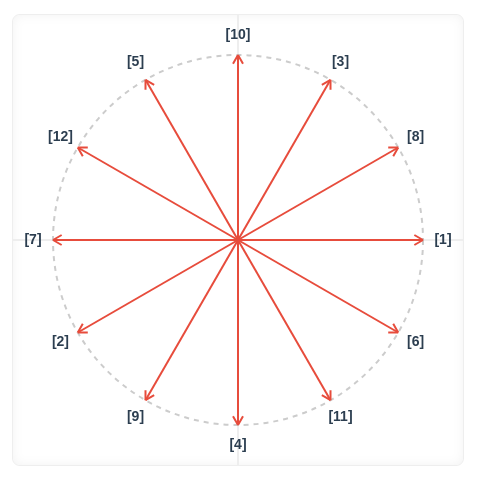
\includegraphics[width=0.55\textwidth]{slot_diagram.png}
    \caption{Star of slots diagram for the 12-slot, 14-pole fractional-slot winding.}
    \label{fig:slot_diagram}
\end{figure}

\subsection*{2. Phasor Diagram and Fundamental Winding Factor}

To maintain a balanced 3-phase machine, the 12 slots must be divided equally among the 3 phases, resulting in 4 slots per phase. The optimal phase allocation is determined by grouping the slot phasors closest to the primary magnetic axes.\\

For Phase A, the slots clustered around $0^\circ$ and $180^\circ$ are grouped as follows:\\
\begin{itemize}
    \item \textbf{Phase A+:} Slot 1 ($0^\circ$) and Slot 8 ($30^\circ$)
    \item \textbf{Phase A-:} Slot 7 ($180^\circ$) and Slot 2 ($210^\circ$)
\end{itemize}

\begin{figure}[H]
    \centering
    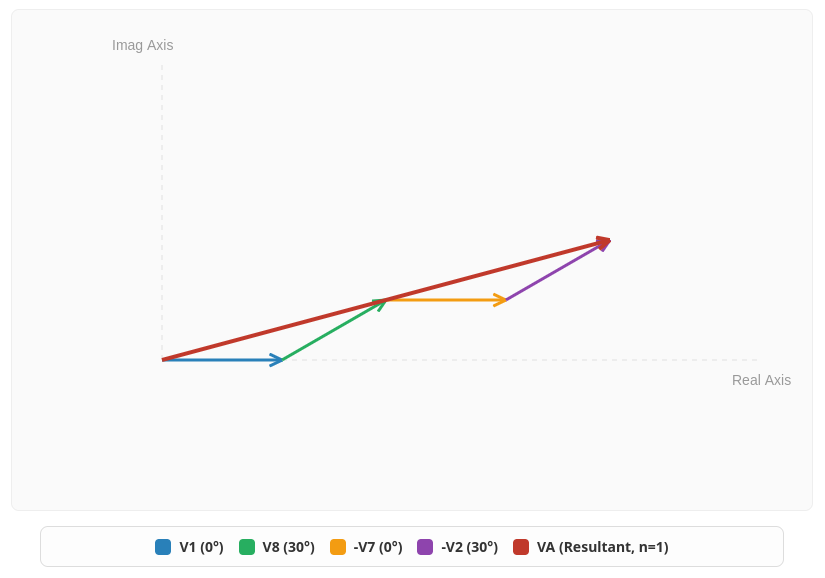
\includegraphics[width=0.55\textwidth]{fundamental_phasor.png}
    \caption{Phasor addition diagram for Phase A fundamental voltage.}
    \label{fig:phasor_fund}
\end{figure}

\subsubsection*{Induced Voltage Calculation}
The total induced voltage for Phase A ($V_A$) is the vector sum of these individual slot voltages. The voltages of the negative return path slots (Slot 7 and Slot 2) are subtracted, which is mathematically equivalent to adding $180^\circ$ to their phase angles.

\begin{align*}
    V_A &= V_1 + V_8 - V_7 - V_2 \\
    V_A &= 1\angle 0^\circ + 1\angle 30^\circ - 1\angle 180^\circ - 1\angle 210^\circ
\end{align*}

After adjusting the negative return paths by $180^\circ$, the geometric sum simplifies to:
$$V_A = 2(1\angle 0^\circ) + 2(1\angle 30^\circ)$$

The resultant voltage is calculated by summing the real and imaginary components of the individual slot vectors:
\begin{align*}
    V_{A,real} &= 2\cos(0^\circ) + 2\cos(30^\circ) \\
    V_{A,real} &= 2(1) + 2\left(\frac{\sqrt{3}}{2}\right) = 2 + \sqrt{3} \approx 3.732 \\
    \\
    V_{A,imag} &= 2\sin(0^\circ) + 2\sin(30^\circ) \\
    V_{A,imag} &= 2(0) + 2\left(\frac{1}{2}\right) = 0 + 1 = 1.0
\end{align*}

The magnitude of the total Phase A voltage is the hypotenuse of the real and imaginary components:
$$|V_A| = \sqrt{V_{A,real}^2 + V_{A,imag}^2} = \sqrt{(3.732)^2 + (1.0)^2} = \sqrt{13.928 + 1.0} = 3.8637$$

\subsubsection*{Winding Factor ($K_{w1}$)}
The fundamental winding factor is defined as the ratio of the actual geometric sum to the arithmetic sum .
$$K_{w1} = \frac{|V_A|}{\text{Number of Slots per Phase}} = \frac{3.8637}{4} = \mathbf{0.9659}$$


\subsection*{3. Harmonic Winding Factors}

The electrical angle for each slot is recalculated for the 3rd and 5th harmonics. The base electrical shift is multiplied by the harmonic number $n$.
\begin{itemize}
    \item \textbf{3rd Harmonic Shift:} $\alpha_{e3} = 3 \cdot 210^\circ = 630^\circ \equiv 270^\circ \pmod{360^\circ}$
    \item \textbf{5th Harmonic Shift:} $\alpha_{e5} = 5 \cdot 210^\circ = 1050^\circ \equiv 330^\circ \pmod{360^\circ}$
\end{itemize}

\vspace{0.3cm}
\begin{table}[H]
\centering
\renewcommand{\arraystretch}{1.2}
\begin{tabular}{ccc}
\toprule
\textbf{Slot ($Q$)} & \textbf{3rd Harmonic Angle} & \textbf{5th Harmonic Angle} \\
\midrule
1 & $\mathbf{0^\circ}$ & $\mathbf{0^\circ}$ \\
2 & $\mathbf{270^\circ}$ & $\mathbf{330^\circ}$ \\
3 & $\mathbf{180^\circ}$ & $\mathbf{300^\circ}$ \\
4 & $\mathbf{90^\circ}$ & $\mathbf{270^\circ}$ \\
5 & $\mathbf{0^\circ}$ & $\mathbf{240^\circ}$ \\
6 & $\mathbf{270^\circ}$ & $\mathbf{210^\circ}$ \\
7 & $\mathbf{180^\circ}$ & $\mathbf{180^\circ}$ \\
8 & $\mathbf{90^\circ}$ & $\mathbf{150^\circ}$ \\
9 & $\mathbf{0^\circ}$ & $\mathbf{120^\circ}$ \\
10 & $\mathbf{270^\circ}$ & $\mathbf{90^\circ}$ \\
11 & $\mathbf{180^\circ}$ & $\mathbf{60^\circ}$ \\
12 & $\mathbf{90^\circ}$ & $\mathbf{30^\circ}$ \\
\bottomrule
\end{tabular}
\caption{Induced voltage phase angles for the 3rd and 5th harmonics.}
\end{table}

\subsubsection*{3rd Harmonic}
The fundamental phase angles are multiplied by 3. Adjustments for the negative return paths are applied after the multiplication.
\begin{itemize}
    \item $V_1$: $0^\circ \cdot 3 = 0^\circ$
    \item $V_8$: $30^\circ \cdot 3 = 90^\circ$
    \item $-V_7$: $(180^\circ \cdot 3) + 180^\circ = 720^\circ \equiv 0^\circ$
    \item $-V_2$: $(210^\circ \cdot 3) + 180^\circ = 810^\circ \equiv 90^\circ$
\end{itemize}

\begin{figure}[H]
    \centering
    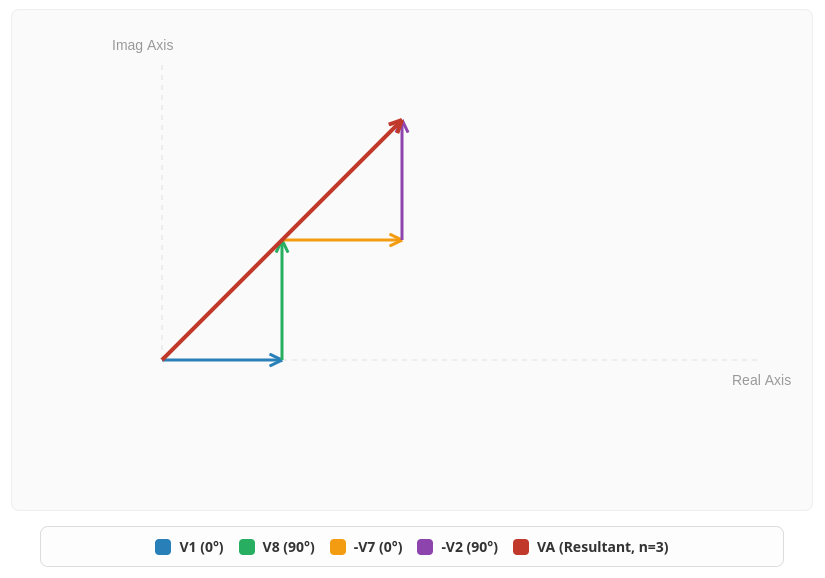
\includegraphics[width=0.55\textwidth]{third_phasor.png}
    \caption{Phasor addition diagram for Phase A 3rd harmonic voltage.}
    \label{fig:phasor_third}
\end{figure}

The geometric sum becomes:
$$V_{A3} = 2(1\angle 0^\circ) + 2(1\angle 90^\circ)$$

Calculating the real and imaginary components:
\begin{align*}
    V_{A3,real} &= 2\cos(0^\circ) + 2\cos(90^\circ) = 2(1) + 2(0) = 2.0 \\
    V_{A3,imag} &= 2\sin(0^\circ) + 2\sin(90^\circ) = 2(0) + 2(1) = 2.0
\end{align*}

The magnitude and corresponding winding factor are:
\begin{align*}
    |V_{A3}| &= \sqrt{(2.0)^2 + (2.0)^2} = \sqrt{8} \approx 2.828 \\
    K_{w3} &= \frac{2.828}{4} = \mathbf{0.7071}
\end{align*}

\subsubsection*{5th Harmonic ($n=5$)}
The fundamental phase angles are multiplied by 5.
\begin{itemize}
    \item $V_1$: $0^\circ \cdot 5 = 0^\circ$
    \item $V_8$: $30^\circ \cdot 5 = 150^\circ$
    \item $-V_7$: $(180^\circ \cdot 5) + 180^\circ = 1080^\circ \equiv 0^\circ$
    \item $-V_2$: $(210^\circ \cdot 5) + 180^\circ = 1230^\circ \equiv 150^\circ$
\end{itemize}

\begin{figure}[H]
    \centering
    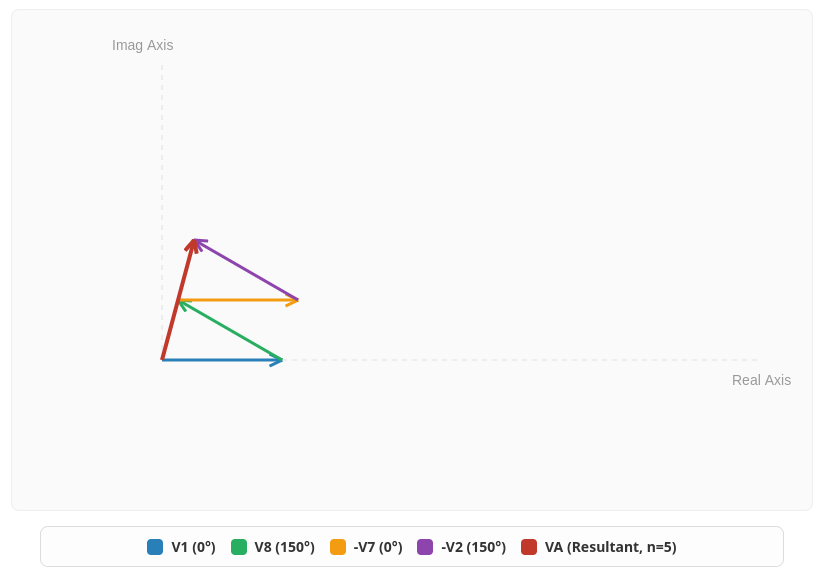
\includegraphics[width=0.55\textwidth]{fifth_phasor.png}
    \caption{Phasor addition diagram for Phase A 5th harmonic voltage.}
    \label{fig:phasor_fifth}
\end{figure}

The geometric sum becomes:
$$V_{A5} = 2(1\angle 0^\circ) + 2(1\angle 150^\circ)$$

Calculating the real and imaginary components:
\begin{align*}
    V_{A5,real} &= 2\cos(0^\circ) + 2\cos(150^\circ) = 2(1) + 2(-0.866) = 2 - 1.732 = 0.268 \\
    V_{A5,imag} &= 2\sin(0^\circ) + 2\sin(150^\circ) = 2(0) + 2(0.5) = 1.0
\end{align*}

The magnitude and corresponding winding factor are:
\begin{align*}
    |V_{A5}| &= \sqrt{(0.268)^2 + (1.0)^2} = \sqrt{0.0718 + 1.0} \approx 1.035 \\
    K_{w5} &= \frac{1.035}{4} = \mathbf{0.2588}
\end{align*}

In this fractional-slot design, the fundamental winding factor ($K_{w1} = 0.9659$) is quite high, showing torque is generated with minimal losses. There is significant 3rd harmonic component however in a star-connected 3-phase machine, these harmonics will naturally cancel out line-to-line, but they can still cause saturation in the core. The 5th harmonic is relatively suppressed ($K_{w5} = 0.2588$), which will reduce rotor eddy current losses.

\subsection*{4. Winding Layout Diagram and Verification}

To complete the 3-phase fractional-slot machine, the remaining 8 slots must be systematically assigned to Phase B and Phase C. In a balanced 3-phase system, the voltages of the phases are electrically separated by $120^\circ$.

\begin{itemize}
    \item \textbf{Phase B ($240^\circ$ offset):} The slots around $240^\circ$ (Slot 9 and Slot 4) are assigned as the positive paths, and the slots around $60^\circ$ (Slot 3 and Slot 10) form the negative return paths.
    \item \textbf{Phase C ($120^\circ$ offset):} The slots around $120^\circ$ (Slot 5 and Slot 12) act as the positive paths, and the slots around $300^\circ$ (Slot 11 and Slot 6) form the negative return paths.
\end{itemize}

\begin{figure}[H]
    \centering
    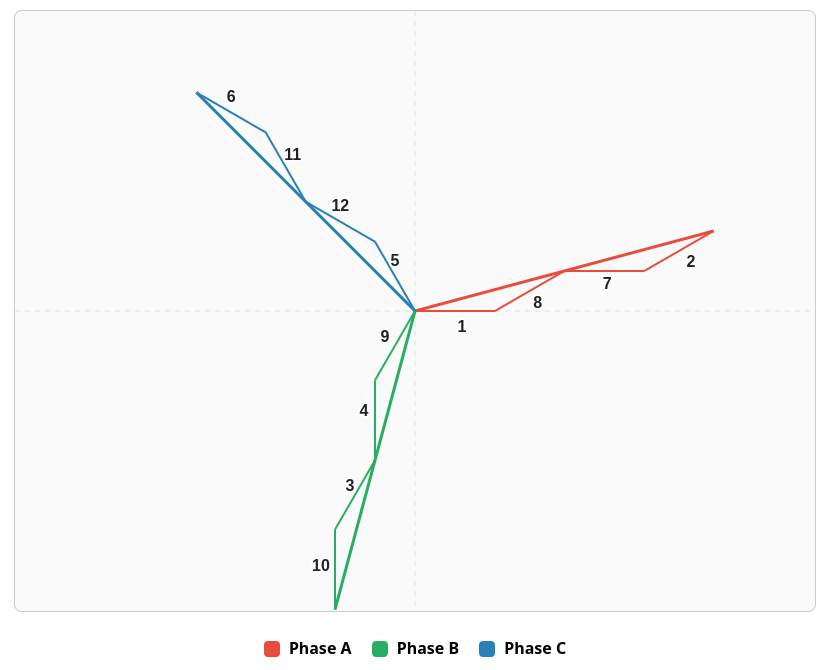
\includegraphics[width=0.65\textwidth]{phase_phasor_diagram.png}
    \caption{Phasor addition diagram demonstrating the geometric $120^\circ$ shift between all three phases.}
    \label{fig:all_phases}
\end{figure}

By mapping these assignments chronologically from Slot 1 to Slot 12, the final physical winding layout of the stator is established.

\vspace{0.3cm}
\begin{table}[H]
\centering
\renewcommand{\arraystretch}{1.3}
\begin{tabular}{|l|*{12}{c|}}
\hline
\textbf{Slot ($Q$)} & \textbf{1} & \textbf{2} & \textbf{3} & \textbf{4} & \textbf{5} & \textbf{6} & \textbf{7} & \textbf{8} & \textbf{9} & \textbf{10} & \textbf{11} & \textbf{12} \\ \hline
\textbf{Phase} & A & -A & -B & B & C & -C & -A & A & B & -B & -C & C \\ \hline
\end{tabular}
\caption{Phase layout mapping for the 12-slot, 14-pole concentrated winding.}
\end{table}

The resulting winding diagram shows a balanced fractional-slot concentrated winding. Each of the three phases occupies 4 slots. Furthermore, the phase diagram shows a symmetrical geometry that guarantees the induced EMFs in Phases A, B, and C are equal in magnitude and precisely shifted by $120^\circ$ electrical from one another.

\end{document}
